\documentclass[professionalfont]{beamer}
%\usecolortheme{default}
\usetheme{Madrid}
\usepackage{subcaption}
\usepackage{caption}
\usepackage{tikz}

\usepackage{pst-all}
\usepackage{leftidx}

\title{\textbf{Chiral Central Charge from a Single Bulk Wave Function}}
\subtitle{I. H. Kim, B. Shi, K. Kato, \& V. V. Albert \\ PRL \textbf{128}, 176402  (2022)}

\author{Chen-Chih Wang}
\institute{NTHU}
\date{December 2, 2025}

\newcommand{\anglelr}[1]{\left\langle #1 \right\rangle}
\newcommand{\abs}[1]{\left| #1 \right|}
\newcommand{\de}{\partial}
\newcommand{\pdif}[1]{\frac{\partial }{\partial #1}}
\newcommand{\pdiff}[2]{\frac{\partial #1}{\partial #2}}
\newcommand{\lr}[1]{\left(#1\right)}
\newcommand{\lrm}[1]{\left[#1\right]}
\newcommand{\lrg}[1]{\left\{#1\right\}}
\newcommand{\lran}[1]{\left\langle #1 \right\rangle}
\newcommand{\lra}[1]{\left|#1\right|}
\newcommand{\ket}[1]{\left| #1 \right\rangle}
\newcommand{\bra}[1]{\left\langle #1 \right|}
\newcommand{\braket}[2]{\left\langle #1 \right|\left. #2\right\rangle}
\newcommand{\mrm}[1]{\mathrm{#1}}
\newcommand{\bo}[1]{\mathbf{#1}}
\newcommand{\gk}{\gamma_{\mathbf{k}}}
\newcommand{\uk}{u_{\mathbf{k}}}
\newcommand{\vk}{v_{\mathbf{k}}}
\newcommand{\vkp}{v_{\mathbf{k}'}}

\newtheorem{axiom}{Axiom}

\newcommand{\wordfig}[2]{\begin{minipage}[h]{#1 cm}
	\vspace{0pt}
	\includegraphics[width=\textwidth]{#2}
   \end{minipage}}
   
\newcommand{\wordfigdir}[2]{
\begin{minipage}[h]{#1 cm}
\centering
	\vspace{0pt}
	#2
\end{minipage}}

%\setbeamercolor{frametitle}{fg=black,bg=blue}
%\setbeamertemplate{frametitle}[default][left]
%\setbeamerfont{frametitle}{size=\huge}
%\setbeamerfont{block title}{size=\Large}

\begin{document}
%%%%%%%%%%%%%%%%%%%%%%%%%%%%%%%%%%%%%%%%%%%%%%%%
\begin{frame}
    \titlepage
\end{frame}
%%%%%%%%%%%%%%%%%%%%%%%%%%%%%%%%%%%%%%%%%%%%%%%%
\begin{frame}
    \begin{itemize}
        \item Phys. Rev. Lett. \textbf{128}, 176402 (2022)
        \item Phys. Rev. B \textbf{106}, 075147 (2022)
        \item Phys. Rev. Lett. \textbf{129}, 260402 (2022)
    \end{itemize}
\end{frame}
%%%%%%%%%%%%%%%%%%  content  %%%%%%%%%%%%%%%%%%%
\begin{frame}{Outline}
   \tableofcontents
\end{frame}
%%%%%%%%%%%%%%%%%%%%%%%%%%%%%%%%%%%%%%%%%%%%%%%%
{
\setbeamercolor{background canvas}{bg=lightgray}
\section{Introduction}
\begin{frame}
    \centering
    \huge
    \textbf{Introduction}
\end{frame}
}
%%%%%%%%%%%%%%%%%%%%%%%%%%%%%%%%%%%%%%%%%%%%%%%%
\subsection{Chiral Central Charge: a brief review}
\begin{frame}{Chiral Central Charge: a brief review}

\begin{itemize}
    \item (1+1)D CFT -- boundary of a (2+1)D gapped bulk.
        
    \item Virasoro algebra
\end{itemize}
\vspace{-0.5cm}
        {\tiny
            \begin{figure}
                \centering
                \begin{minipage}{0.45\linewidth}
                    \[
                    \left\{
                    \begin{aligned}
                        & T(z) := T_{00} - T_{11} + 2iT_{01} = \sum_{n\in\mathbb{Z}}\frac{1}{z^{n+2}}L_n\\
                        & \overline{T}(\bar{z}):= T_{00} - T_{11} - 2iT_{01} = \sum_{n\in\mathbb{Z}}\frac{1}{\bar{z}^{n+2}}\overline{L}_n
                    \end{aligned}
                    \right.
                    \]
                \end{minipage}
                \begin{minipage}{0.45\linewidth}
                    \[\left\{
                    \begin{aligned}
                    & [L_n,L_m] = (n-m)L_{n+m}+\frac{1}{12}\alert{\boldsymbol{c}}(n^3-n)\delta_{n,-m} \\
                    & [\overline{L}_n,\overline{L}_m] = (n-m)\overline{L}_{n+m}+\frac{1}{12}\boldsymbol{\alert{\overline{c}}}(n^3-n)\delta_{n,-m} \\
                    & [L_n,\overline{L}_m]=0
                    \end{aligned}
                    \right.\]
                \end{minipage}
            \end{figure}
        }

\begin{itemize}
    \item Chiral central charge (CCC): $c_-:=c-\overline{c}$.
    \item Edge current: $I = \frac{\pi}{12}c_- T^2$
\end{itemize}

\begin{figure}
    \centering
    \begin{minipage}{0.5\linewidth}
        \begin{figure}
            \centering
            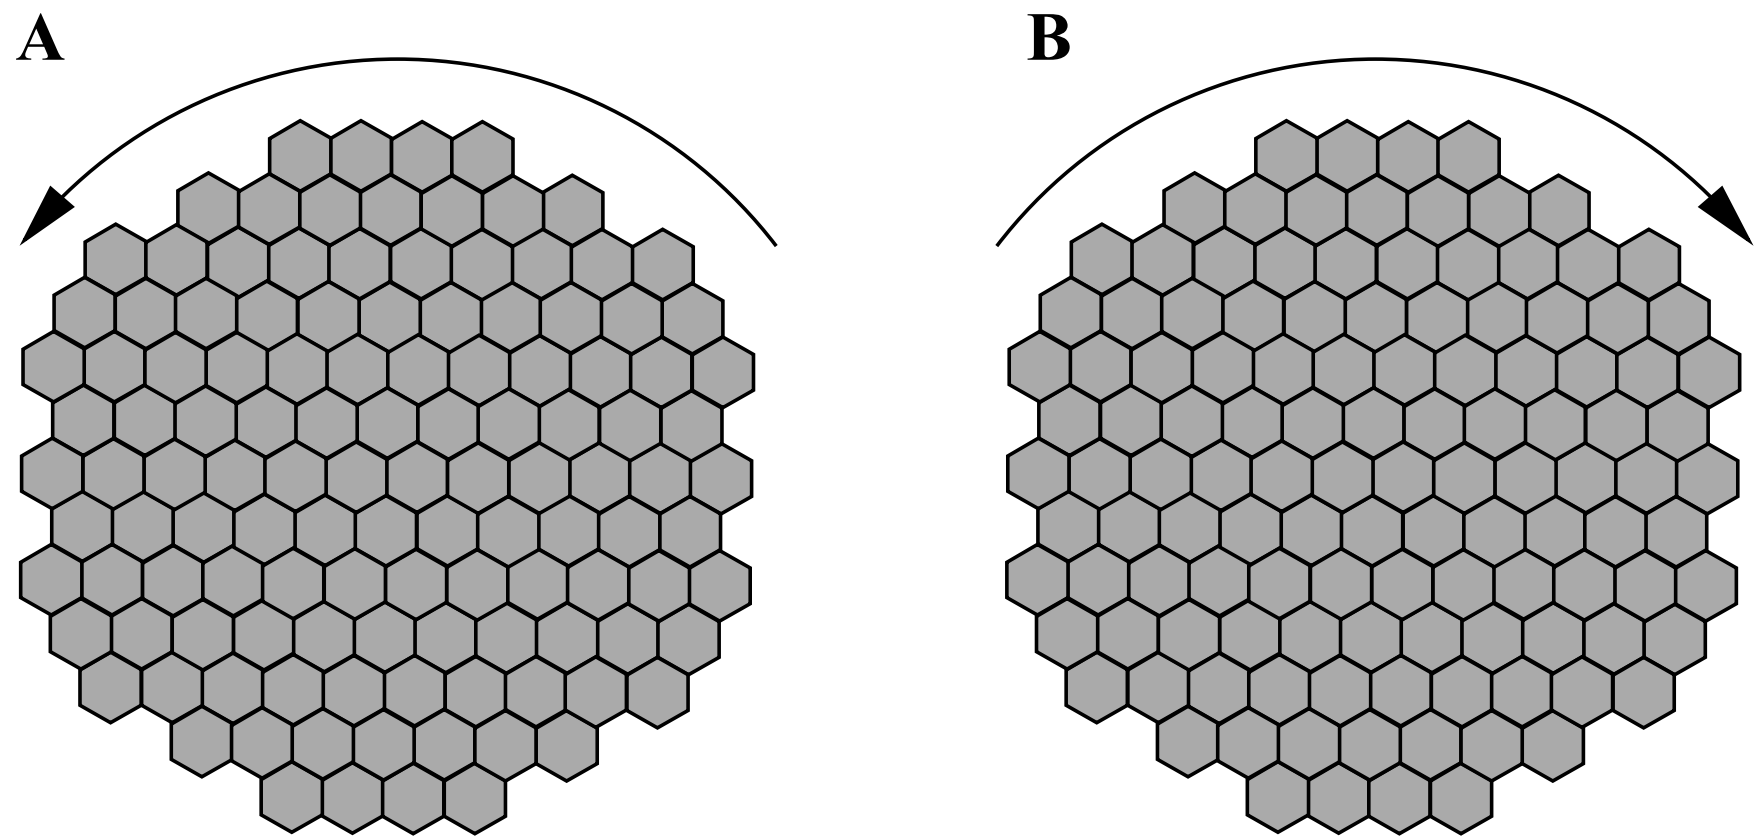
\includegraphics[width=0.9\linewidth]{edge-mode.png}
        \end{figure}
    \end{minipage}
    \begin{minipage}{0.45\linewidth}
        {
        \tiny
        \begin{itemize}
            \item A. Cappelli et al., Nucl. Phys. B \textbf{636}, 568 (2002)
            \item A. Kitaev, Ann. Phys. \textbf{321}, 2 (2006)
        \end{itemize}
        }
    \end{minipage}
\end{figure}

\end{frame}
%%%%%%%%%%%%%%%%%%%%%%%%%%%%%%%%%%%%%%%%%%%%%%%%
\subsection{Motivations}
\begin{frame}{Motivations}
\textbf{Topological ordered states:}
\begin{figure}
    \centering
    \begin{minipage}{0.5\linewidth}
        \begin{itemize}
            \item Topological entanglement entropy
            \item Entanglement spectrum
            \item Topological $S$ and $T$ matrices (mutual- and self-statistics)
        \end{itemize}
    \end{minipage}
    \begin{minipage}{0.4\linewidth}
        \begin{equation*}
            \begin{aligned}
            &S_{ab} = \frac{1}{\mathcal{D}}
            \wordfigdir{1.4}{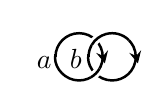
\begin{tikzpicture}[scale=0.6]
              % centers and radius (for reference)
              % left center = (0.9,0.7), right center = (1.6,0.7), r = 0.5
              % intersection angles (approx):
              % left: upper ~ 45.573°, lower ~ 314.427°
              % right: upper ~ 134.427°, lower ~ 225.573°
            
              % --- Base arcs (thin strokes, include arrow heads) ---
              % Left: long arrowed path (keeps orientation like your PSTricks)
              \draw[line width=0.9pt, -<, >=stealth, shorten <=1pt]
                (0.9,0.7) ++(167:0.5) arc[start angle=167, end angle=373, radius=0.5];
            
              % Left: top semic (like your original \psarc 0..180)
              \draw[line width=0.9pt]
                (0.9,0.7) ++(0:0.5) arc[start angle=0, end angle=180, radius=0.5];
            
              % Right: long arrowed path
              \draw[line width=0.9pt, -<, >=stealth, shorten <=1pt]
                (1.6,0.7) ++(167:0.5) arc[start angle=167, end angle=373, radius=0.5];
            
              % Right: small filler arcs (as in the PSTricks original)
              \draw[line width=0.9pt]
                (1.6,0.7) ++(0:0.5) arc[start angle=0, end angle=50, radius=0.5];
              \draw[line width=0.9pt]
                (1.6,0.7) ++(145:0.5) arc[start angle=145, end angle=180, radius=0.5];
            
              % --- Overpasses (draw AFTER base strokes, use preaction to mask underlying lines)
              % Right circle should pass OVER at the UPPER intersection:
              % draw the right circle's upper arc with a white preaction so it appears on top there.
              \draw[line width=0.9pt,
                    preaction={draw, line width=3pt, white}]
                (1.6,0.7) ++(45:0.5) arc[start angle=45, end angle=150, radius=0.5];
            
              % Left circle should pass OVER at the LOWER intersection:
              % draw a short left-circle arc around the lower intersection with preaction.
              % choose a segment centered at the computed lower angle ~314.43° (we use 300..330°)
              \draw[line width=0.9pt,
                    preaction={draw, line width=3pt, white}]
                (0.9,0.7) ++(300:0.5) arc[start angle=300, end angle=330, radius=0.5];
            
              % (Optionally draw a slightly larger left overpass if you want a wider 'over' region)
              %\draw[line width=0.9pt, preaction={draw, line width=3pt, white}]
              %  (0.9,0.7) ++(295:0.5) arc[start angle=295, end angle=335, radius=0.5];
            
              % --- Labels (same placement as original) ---
              \node[anchor=base west] at (-0.2,0.45) {$a$};
              \node[anchor=base west] at (0.5,0.45) {$b$};
            \end{tikzpicture}}
            \\
            &\begin{aligned}
            T_{ab} &= \theta_a\delta_{ab} \\
            &= 
            \frac{1}{d_a}
            \wordfigdir{1.8}{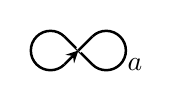
\begin{tikzpicture}[scale=0.5]
            % Base settings
            \tikzset{
              myarc/.style={line width=0.9pt},
              myline/.style={line width=0.9pt},
              over/.style={preaction={draw, line width=2.3pt, white}}
            }
            
            % --- Arcs ---
            \draw[myarc]
              (0.7071,0) ++(-135:0.5) arc[start angle=-135, end angle=135, radius=0.5];
            
            \draw[myarc]
              (-0.7071,0) ++(45:0.5) arc[start angle=45, end angle=315, radius=0.5];
            
            % --- Straight segments ---
            % Under-passing segment
            \draw[myline]
              (-0.3536,0.3536) -- (0.3536,-0.3536);
            
            % Over-passing segment with arrow
            \draw[myline, over, -{stealth[scale=1.5]}]
              (-0.3536,-0.3536) -- (0,0);
            
            % Over-passing continuation (no arrow)
            \draw[myline, over]
              (0,0) -- (0.3536,0.3536);
            
            % --- Label ---
            \node[anchor=base west] at (1,-0.5) {$a$};
            
            \end{tikzpicture}
            }
            \delta_{ab}
            \end{aligned}
            \end{aligned}
        \end{equation*}
    \end{minipage}
\end{figure}


 \pause

\textbf{Missing piece: Chiral Central Charge (CCC)}
\vspace{-0.4cm}
\begin{figure}
    \begin{minipage}{0.5\linewidth}
    \begin{itemize}
        \item Gapless edge excitations
        \item TRS breaking
        \item Bulk-boundary correspondence
    \end{itemize}
    \end{minipage}
    \begin{minipage}{0.4\linewidth}
        \[
    \underbrace{\frac{1}{\mathcal{D}}\sum_{a}d_a^2
    \theta_a}_{\text{bulk}} = \underbrace{e^{2\pi i c_-/8}}_{\text{boundary}}
    \]
    \end{minipage}
\end{figure}

 

\textbf{Question}: \textbf{A succinct closed-form formula that relates CCC to the ground state entanglement of a single wave function is missing.}
\end{frame}
%%%%%%%%%%%%%%%%%%%%%%%%%%%%%%%%%%%%%%%%%%%%%%%%
\begin{frame}{Motivation}
\begin{figure}
\centering
    \begin{minipage}{0.55\linewidth}
        \textbf{Strategy:} devise a quantity with
        \begin{itemize}
            \item TRS odd
            \item Loop nature (chiral) $\Rightarrow$ Tripartition
            \item Entanglement Hamiltonian
            \item Topological invariant
            \item Energy current $I_{v\to u} = i\anglelr{[h_u,h_v]}$
        \end{itemize}
    \end{minipage}
    \hspace{0.2cm}
    \begin{minipage}{0.4\linewidth}
        \begin{figure}
            \centering
            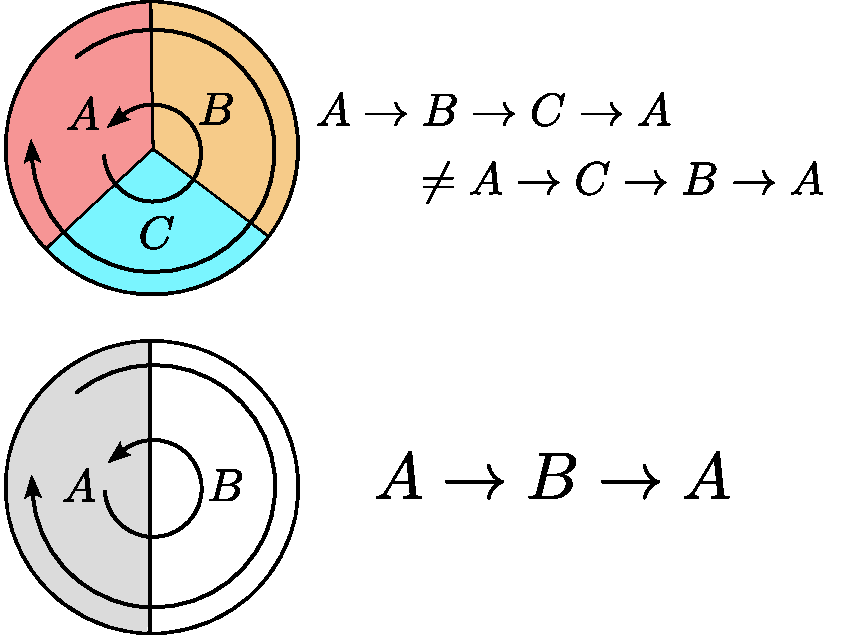
\includegraphics[width=0.9\linewidth]{chiral-at-least-three.pdf}
        \end{figure}
    \end{minipage}
\end{figure}

\begin{definition}[Modular commutator]
    \[J(A,B,C) := i\mrm{Tr}\lr{\rho_{ABC}[K_{AB},K_{BC}]} = i\anglelr{[K_{AB},K_{BC}]}\in \mathbb{R}\]
\end{definition}
    {\small
    $K_X \equiv -\ln\rho_X$ is the entanglement Hamiltonian of the subsystem $X$.
    }
    \pause
\vspace{0.3cm}
    {\small
    \[
    J(A,B,C)_{\rho*} = i\mrm{Tr}\lr{\rho_{ABC}^*\lrm{K_{AB}^*,K_{BC}^*}} = i\lr{-iJ(A,B,C)_\rho}^* = -J(A,B,C)_\rho
    \]
    }
\end{frame}
%%%%%%%%%%%%%%%%%%%%%%%%%%%%%%%%%%%%%%%%%%%%%%%%
{
\setbeamercolor{background canvas}{bg=lightgray}
\section{Methods and Results}
\begin{frame}
    \centering
    \huge
    \textbf{Methods and Results}
\end{frame}
}
%%%%%%%%%%%%%%%%%%%%%%%%%%%%%%%%%%%%%%%%%%%%%%%%
\subsection{Quantum Markov Chain}
\begin{frame}{Quantum Markov Chain}
    \begin{definition}[conditional mutual information]
        \[
        I(A:C|B) := S_{AB}+S_{BC}-S_{B}-S_{ABC}
        \]
    \end{definition}
    {\footnotesize
    Recall that $I(A:C):=S_A+S_C-S_{AC}$, we have
    \begin{align*}
        I(A:C|B) &= I(A:BC)-I(A:B) = I(C:AB)-I(C:B)\\
        &= I(AB:BC)-S_B
    \end{align*}    }
    A \textbf{quantum Markov chain} is a state with the tripartition $A,B,C$ with $I(A:C|B)=0$.
    \vspace{-0.1cm}
    \begin{theorem}[D. Petz (2003)]
    \[
    I(A:C|B) = 0 \Leftrightarrow K_{ABC} = K_{AB} + K_{BC} - K_{B}
    \]
    \end{theorem}
{
\tiny
\begin{itemize}
    \item D. Petz, Rev. Math. Phys. \textbf{15}, 79 (2003)
\end{itemize}
}
This theorem will be used to decompose the entanglement Hamiltonians.
\end{frame}
%%%%%%%%%%%%%%%%%%%%%%%%%%%%%%%%%%%%%%%%%%%%%%%%
\begin{frame}{Quantum Markov Chain}

    {\large
    An important fact is that \textit{the modular commutator vanishes if the state $\rho$ together with the tripartition $A,B,C$ is a quantum Markov chain}.
    }

     

\vspace{0.5cm}

    Because
    \[
    I(A:C|B) = 0 \Leftrightarrow K_{ABC} = K_{AB} + K_{BC} - K_{B}
    \]
then, if the state is a quantum Markov chain, then 
    \begin{align*}
        J(A,C,B)& = i\mrm{Tr}\lr{\rho_{ABC}[K_{AB},K_{BC}]} \\
        &= i\mrm{Tr}\lr{\rho_{ABC}[K_{AB},\lr{K_{ABC}-K_{AB}+K_B}]} \\
        &= i\mrm{Tr}\lr{\rho_{ABC}[K_{AB},K_{ABC}]} + i\mrm{Tr}\lr{\rho_{AB}[K_{AB},K_B]} \\
        &= 0
    \end{align*}
\end{frame}
%%%%%%%%%%%%%%%%%%%%%%%%%%%%%%%%%%%%%%%%%%%%%%%%
\subsection{Area Law}
\begin{frame}{Area Law}
\begin{figure}
    \centering
    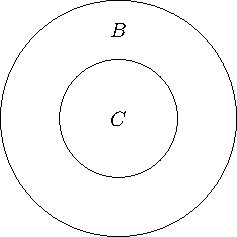
\includegraphics[width=0.3\linewidth]{figure_2.pdf}
\end{figure}
    \begin{axiom}[A0]
    For any state $\sigma$, for any configuration of subsystems $B$ (boundary) together with $C$ (core) topologically equivalent to concentric circles,
    \[
    S(\sigma_{BC}) = S(\sigma_{B}) - S(\sigma_{C})
    \]
    \end{axiom}
\end{frame}
%%%%%%%%%%%%%%%%%%%%%%%%%%%%%%%%%%%%%%%%%%%%%%%%
\begin{frame}{Area Law}

{
\Large
Area law: $S = \alpha l-\gamma$
}
\vspace{0.2cm}
    \begin{figure}
        \centering
        \begin{minipage}{0.3\linewidth}
        \centering
            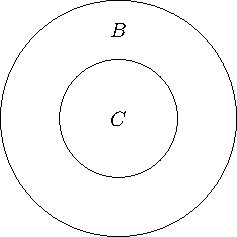
\includegraphics[width=0.7\linewidth]{figure_2.pdf}
        \end{minipage}
        \begin{minipage}{0.5\linewidth}
            \[\left\{
            \begin{aligned}
            &S_B = \alpha\lr{l_1+l_2}-2\gamma \\
            &S_C = \alpha l_1-\gamma\\
            &S_B = \alpha l_2-\gamma
            \end{aligned}\right.
            \]
            \[
            \Rightarrow S_{BC}+S_C=S_B
            \]
        \end{minipage}
    \end{figure}
     
\vspace{0.5cm}
Let $E$ be the environment that purifies the state,
\[
I(E:C) \equiv S_E+S_C-S_{EC} = S_{BC} + S_C - S_B = 0
\]
For any subspace $A\subset E$ of the environment, the subadditivity implies,
\[
I(A:C) \leq I(E:C) = 0
\]

\end{frame}
%%%%%%%%%%%%%%%%%%%%%%%%%%%%%%%%%%%%%%%%%%%%%%%%
\begin{frame}{Area Law}
\begin{figure}
    \centering
    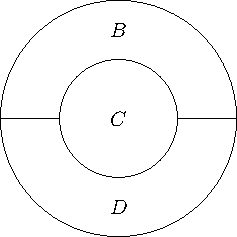
\includegraphics[width=0.3\linewidth]{figure_3.pdf}
\end{figure}
    \begin{axiom}[A1]
        For any state $\sigma$, for any configuration of subsystems $B,D$ (two subsystems that bipartite the boundary) together with $C$ (core), topologically equivalent to the above figure,
        \[
        S(\sigma_{BC}) + S(\sigma_{CD}) - S(\sigma_{B}) - S(\sigma_{D}) = 0
        \]
    \end{axiom}
\end{frame}
%%%%%%%%%%%%%%%%%%%%%%%%%%%%%%%%%%%%%%%%%%%%%%%%
\subsection{Quantum Markov Chain from Area Law}
\begin{frame}{Quantum Markov Chain from Area Law}

{\small
    \begin{figure}
        \centering
        \begin{minipage}{0.4\linewidth}
            \begin{figure}
                \centering
                 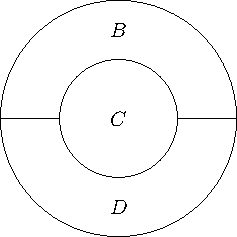
\includegraphics[width=0.7\linewidth]{figure_3.pdf}
            \end{figure}
        \end{minipage}
        \begin{minipage}{0.5\linewidth}
            From Axiom \textbf{A1}, we have
            \begin{align*}
                &S_{BC}+S_{CD}-S_B-S_D\\
                =&S_{BC}+S_{EB}-S_B-S_{EBC}\\
                =& I(E:C|B) =0
            \end{align*}
            Where $E$ is the purifying environment.
        \end{minipage}
    \end{figure}
Let $A\subset E$ be a space outside the system, according to the \textit{subadditivity of the entropy}, we have
\[I(A:C|B)\leq I(E:C|B) = 0\]
That is to say
\[
\text{Axiom A1}\Rightarrow I(A:C|B)=0\stackrel{\mbox{Petz}}\Longrightarrow K_{ABC} = K_{AB}+K_{BC}-K_B
\]
 
\vspace{-0.4cm}
\begin{itemize}
    \item \textbf{Area law} (Axiom \textbf{A1}) implies \textbf{quantum Markov chain}.
    \item The Entanglement Hamiltonian can be decomposed into smaller supports.
\end{itemize}
}
\end{frame}
%%%%%%%%%%%%%%%%%%%%%%%%%%%%%%%%%%%%%%%%%%%%%%%%
\subsection{Decomposition of Entanglement Hamiltonian}
\begin{frame}{Decomposition of Entanglement Hamiltonian}
    \begin{figure}
        \centering
        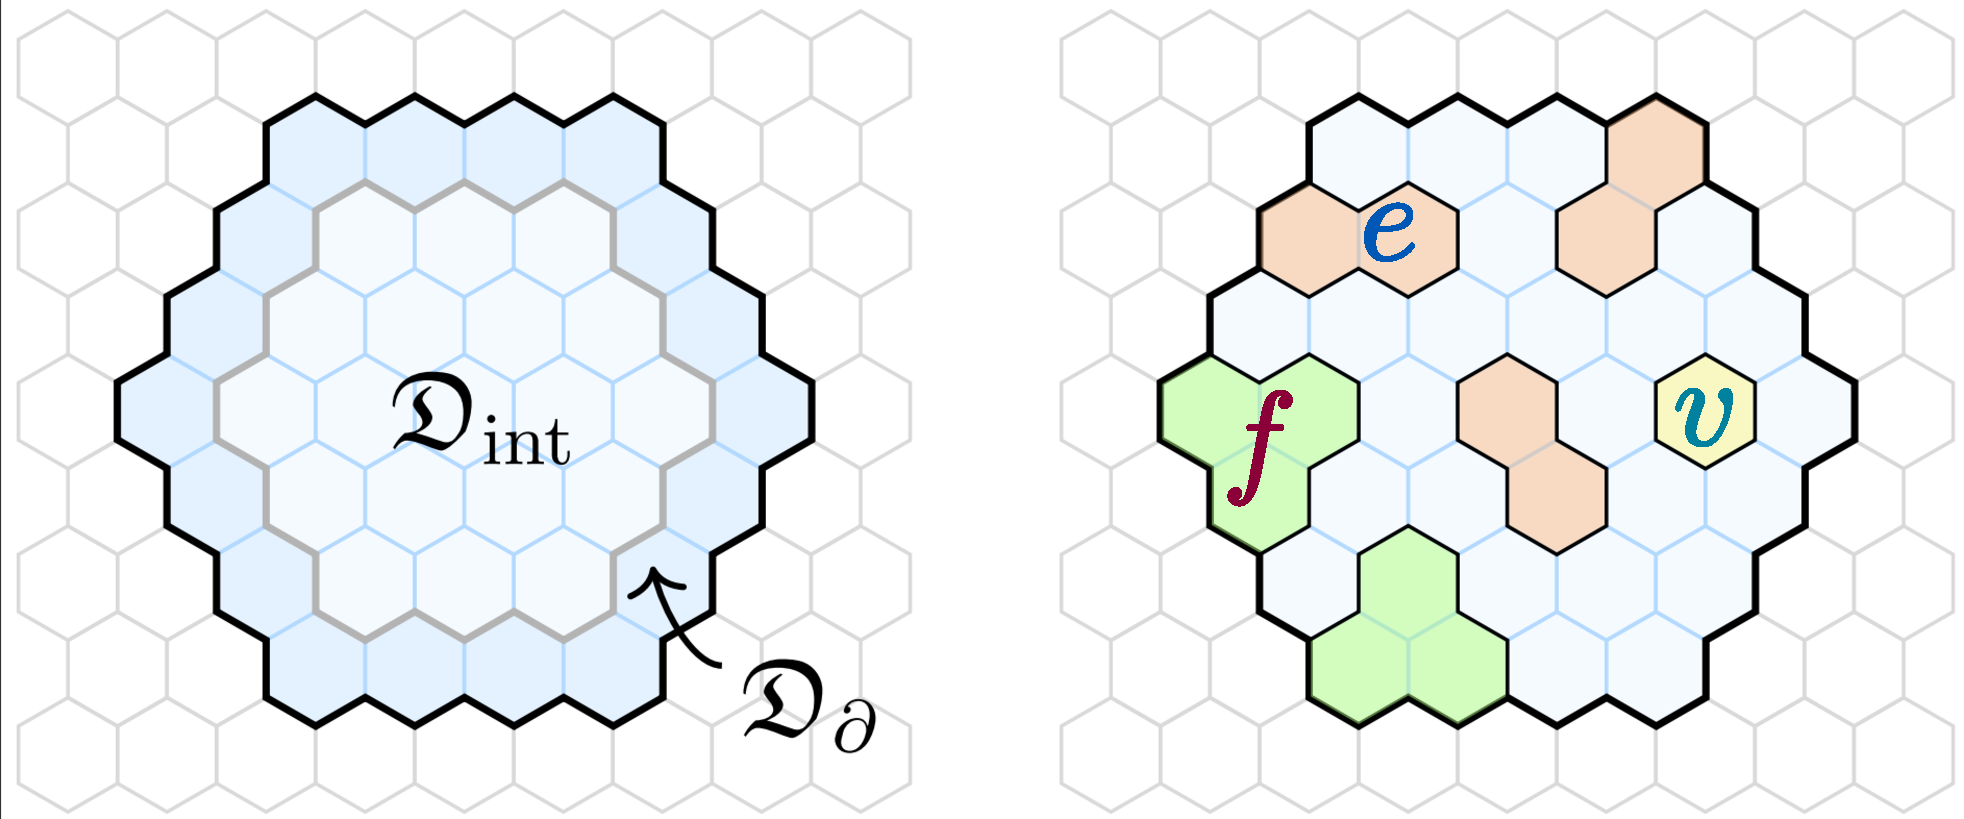
\includegraphics[width=0.6\linewidth]{disk.pdf}
    \end{figure}
    $K_{\mathfrak{D}}$ is the entanglement Hamiltonian of a disk $\mathfrak{D}$. 
     
    \begin{itemize}
        \item Coarse-grain the system into a triangular lattice of supersites.
         
        \item The area law allows us to decompose the entanglement Hamiltonian using the quantum Markov chain trick.
         
        \item Three types, $f$ (face), $e$ (edge), and $v$ (vertex), of subsystems cannot be separated further by the quantum Markov chain trick.
    \end{itemize}
\end{frame}
%%%%%%%%%%%%%%%%%%%%%%%%%%%%%%%%%%%%%%%%%%%%%%%%
\begin{frame}{Decomposition of Entanglement Hamiltonian}
    \begin{figure}
        \centering
         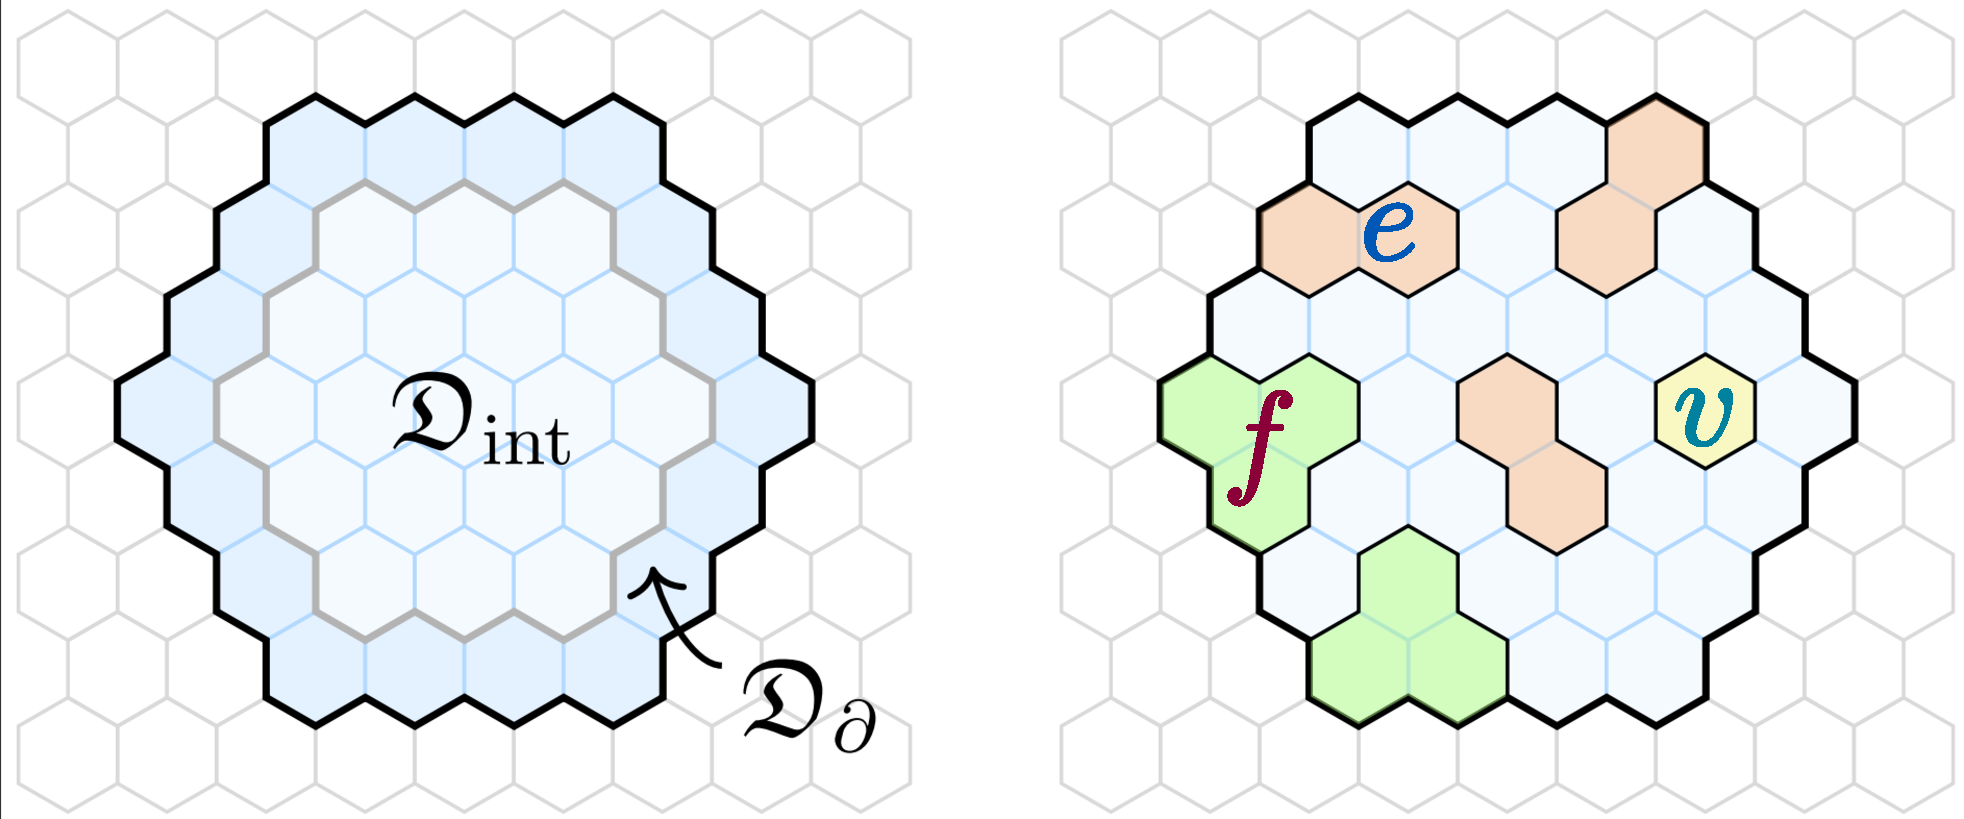
\includegraphics[width=0.4\linewidth]{disk.pdf}
        \hspace{0.5cm}
        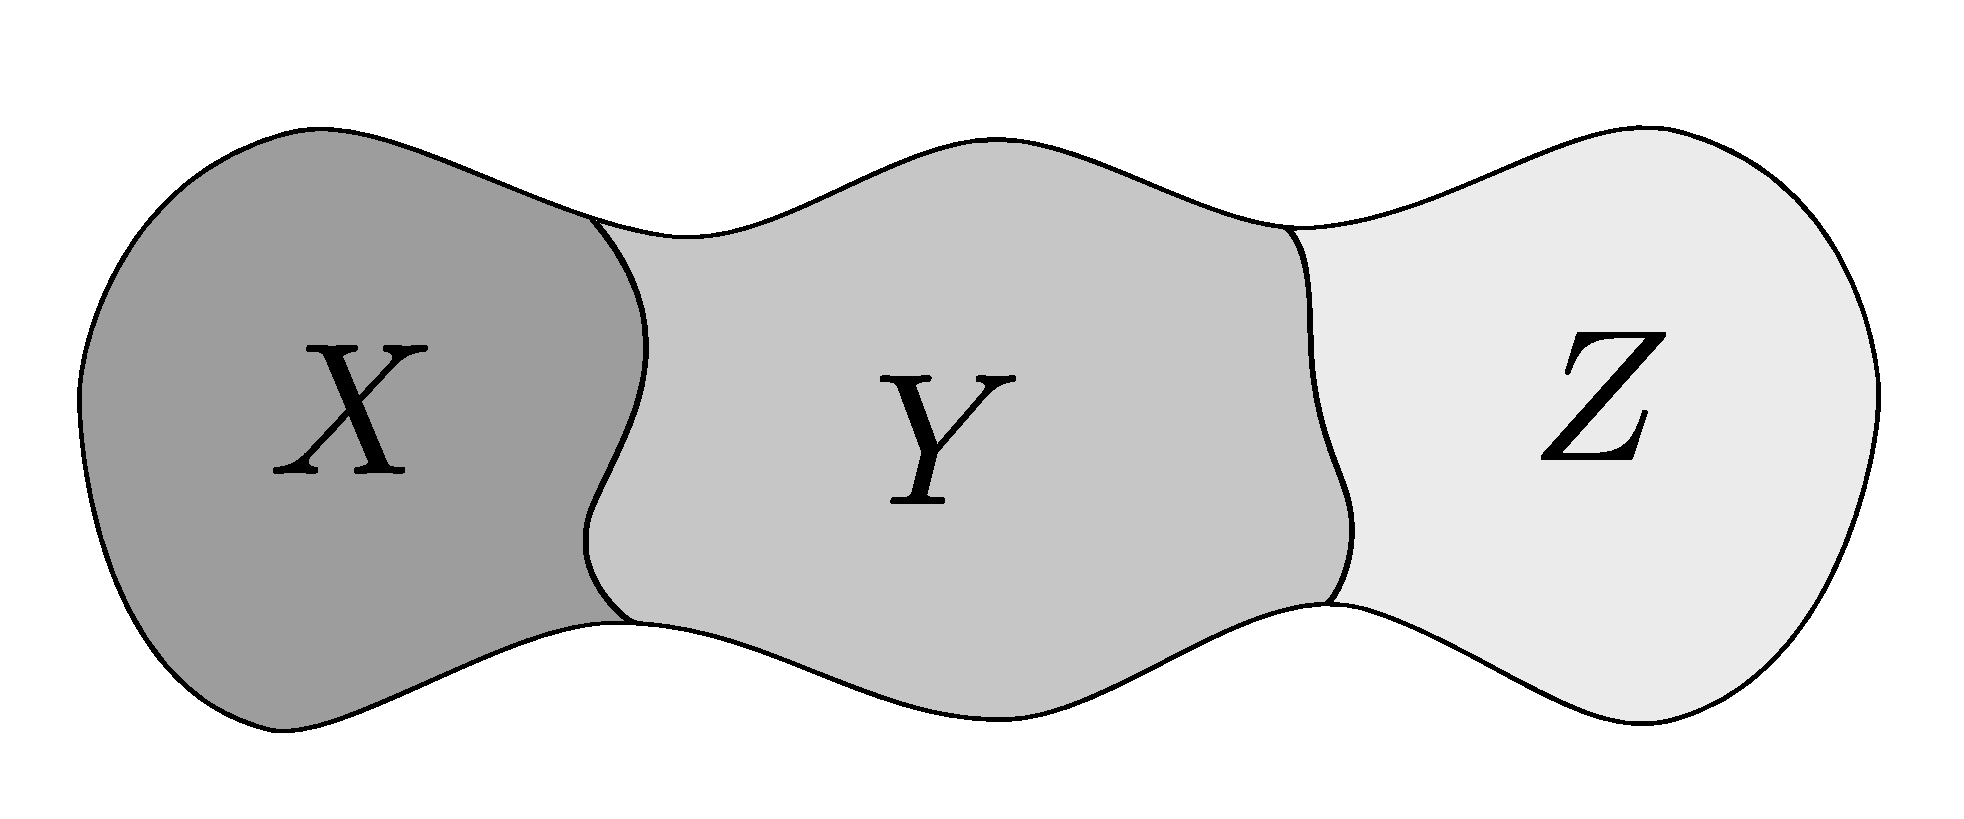
\includegraphics[width=0.4\linewidth]{decomposition.pdf}
    \end{figure}
{
\textbf{Decomposition procedure}
}
\begin{itemize}
    \item Do coarse-graining to define elementary subsystems.  
     
    \item $X$ and $Z$ are disconnected, but both of them are connected to $Y$.
     
    \item Area law axiom implies $I\lr{X:Z|Y}=0$, thus $K_{XYZ} = K_{XY} + K_{YZ} - K_Y$.
     
    \item Continue the process until only $f$, $e$ and $v$ remain.
\end{itemize}
 

Eventually, we will have:
    \[
    K_{\mathfrak{D}} = \sum_{f\in F\lr{\mathfrak{D}}}K_f - \sum_{e\in E\lr{\mathfrak{D}}\setminus E\lr{\mathfrak{D}_\de}}K_e + \sum_{v\in\mathfrak{D}_{\mrm{int}}}K_e
    \]
\end{frame}
%%%%%%%%%%%%%%%%%%%%%%%%%%%%%%%%%%%%%%%%%%%%%%%%
\subsection{Energy Current and Modular Current}
\begin{frame}{Energy Current and Modular Current}
\begin{figure}
    \centering
    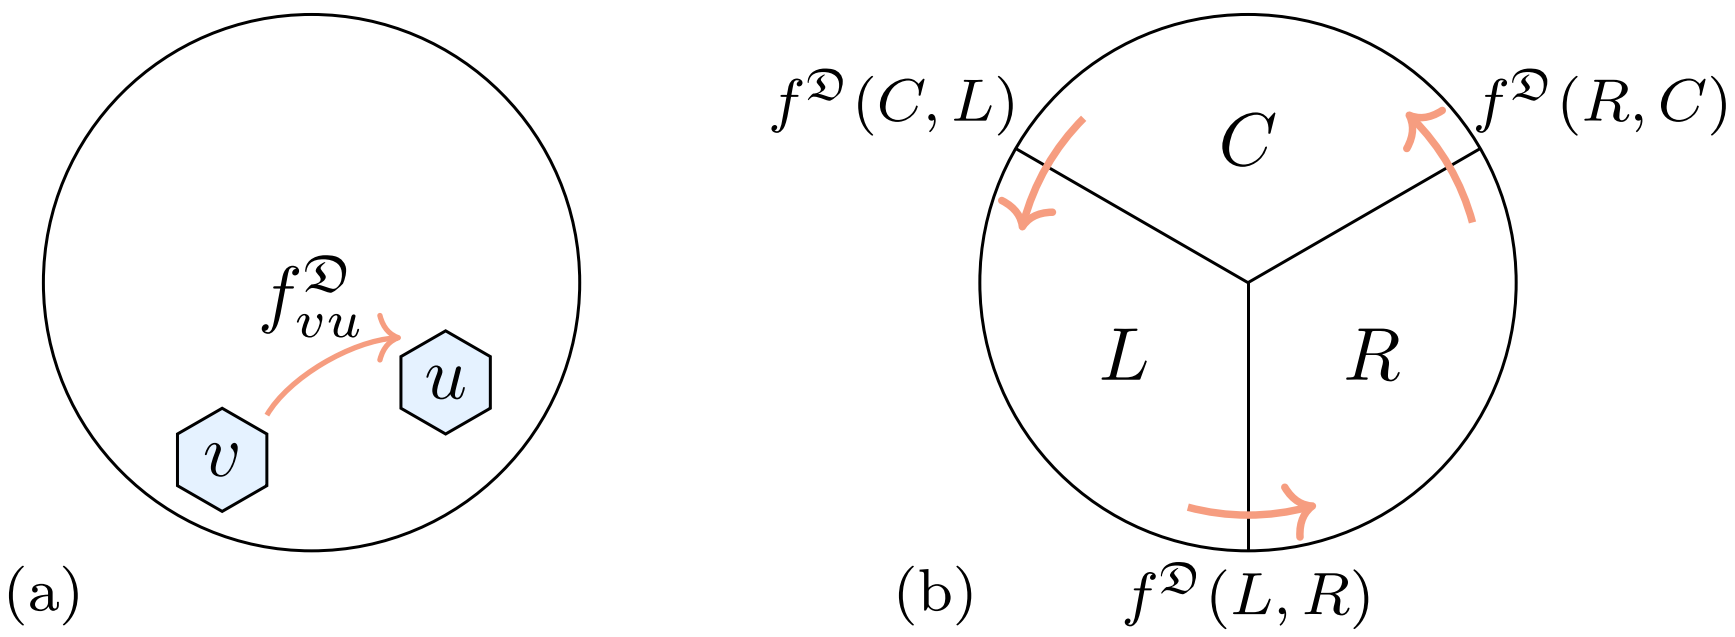
\includegraphics[width=0.6\linewidth]{modular-current.png}
\end{figure}
{\small
    Suppose the Hamiltonian describing the system is local, $H = \sum_{u}h_u$
    \[
    \pdif{t}\anglelr{h_u} = -i\lr{\lrm{H,h_u}} = \sum_{v}i\anglelr{[h_u,h_v]} \equiv \sum_{v}I_{v\to u} = -\oint_u\bo{J}\cdot\mrm{d}\bo{S}
    \]
    then we can follow this to define the energy current from $u$ to $v$ as 
    \[
    I_{v\to u} = i\anglelr{[h_u,h_v]}
    \]
}
\end{frame}
%%%%%%%%%%%%%%%%%%%%%%%%%%%%%%%%%%%%%%%%%%%%%%%%
\begin{frame}{Energy Current and Modular Current}
\begin{figure}
    \centering
    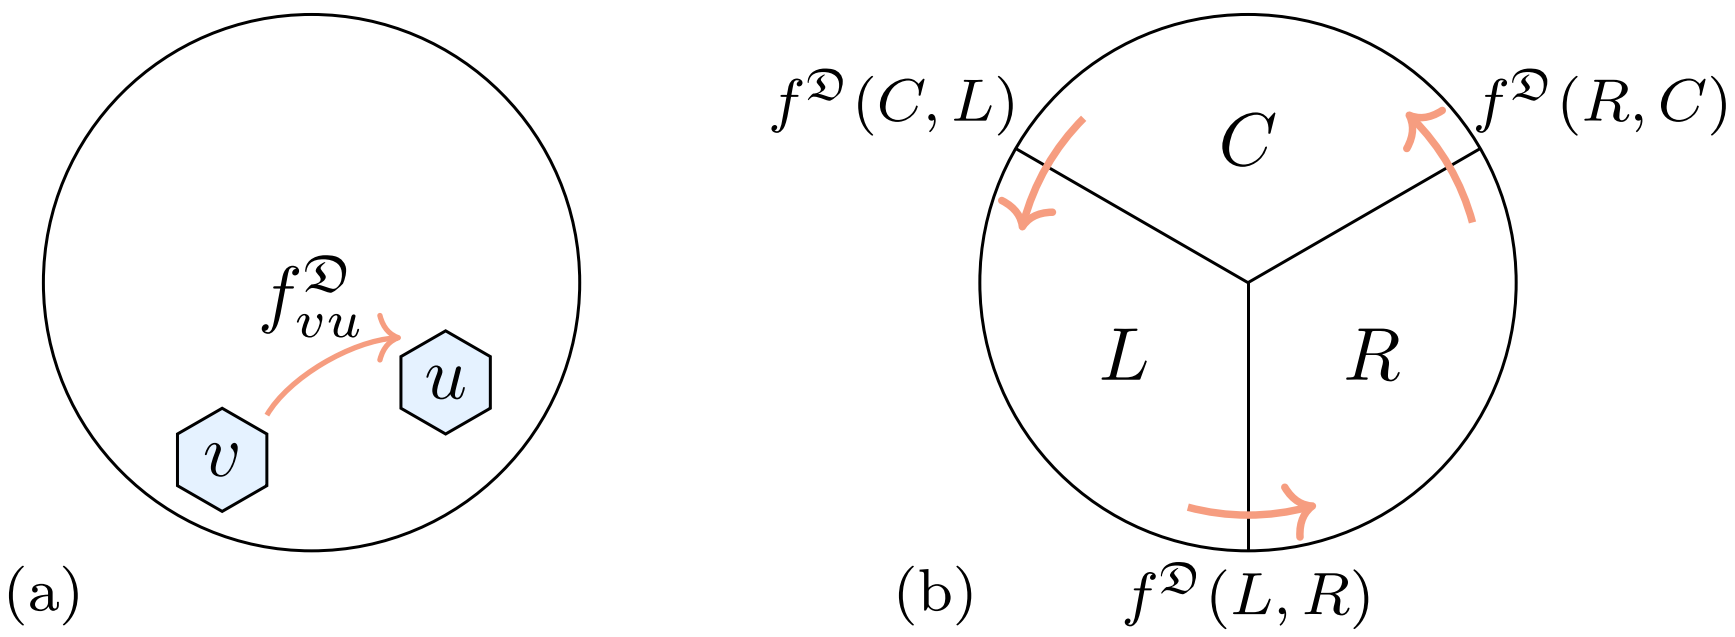
\includegraphics[width=0.6\linewidth]{modular-current.png}
\end{figure}
{\small
Therefore, the modular current is defined in the same way,
    \[
    f^{\mathfrak{D}}_{v\to u}:= i\anglelr{\lrm{\tilde{K}_v^{\mathfrak{D}},\tilde{K}_u^{\mathfrak{D}}}} \quad,\quad f^{\mathfrak{D}}\lr{L,R} := \sum_{v\in L}\sum_{u\in R}f^{\mathfrak{D}}_{v\to u}
    \]
where $\tilde{K}_v^\mathfrak{D}$ collects all terms whose support contains site $v$,
\[
    K_{\mathfrak{D}} = \sum_{f\in F\lr{\mathfrak{D}}}K_f - \sum_{e\in E\lr{\mathfrak{D}}\setminus E\lr{\mathfrak{D}_\de}}K_e + \sum_{v\in\mathfrak{D}_{\mrm{int}}}K_e
    \Rightarrow \sum_{v\in\mathfrak{D}}\tilde{K}_{v}^\mathfrak{D}
    \]
}
    
\end{frame}
%%%%%%%%%%%%%%%%%%%%%%%%%%%%%%%%%%%%%%%%%%%%%%%%
\begin{frame}{Energy Current and Modular Current}
\begin{figure}
    \centering
    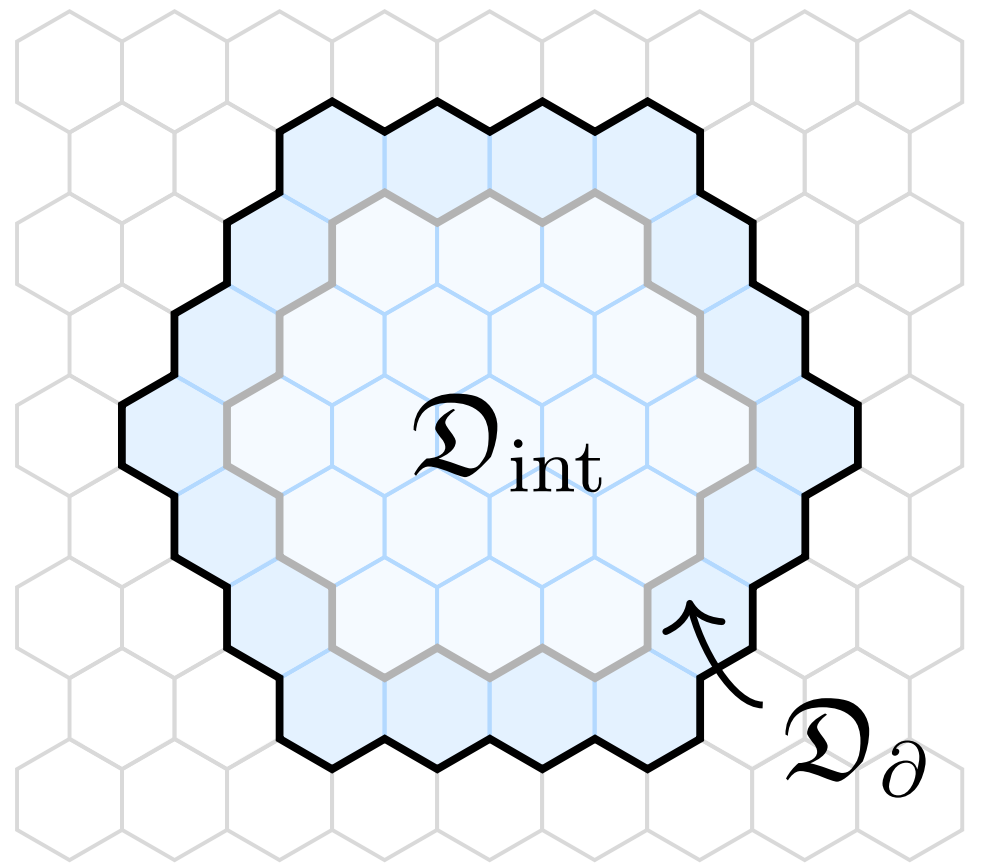
\includegraphics[height=0.2\linewidth]{int-boundary.png}
    \hspace{0.5cm}
    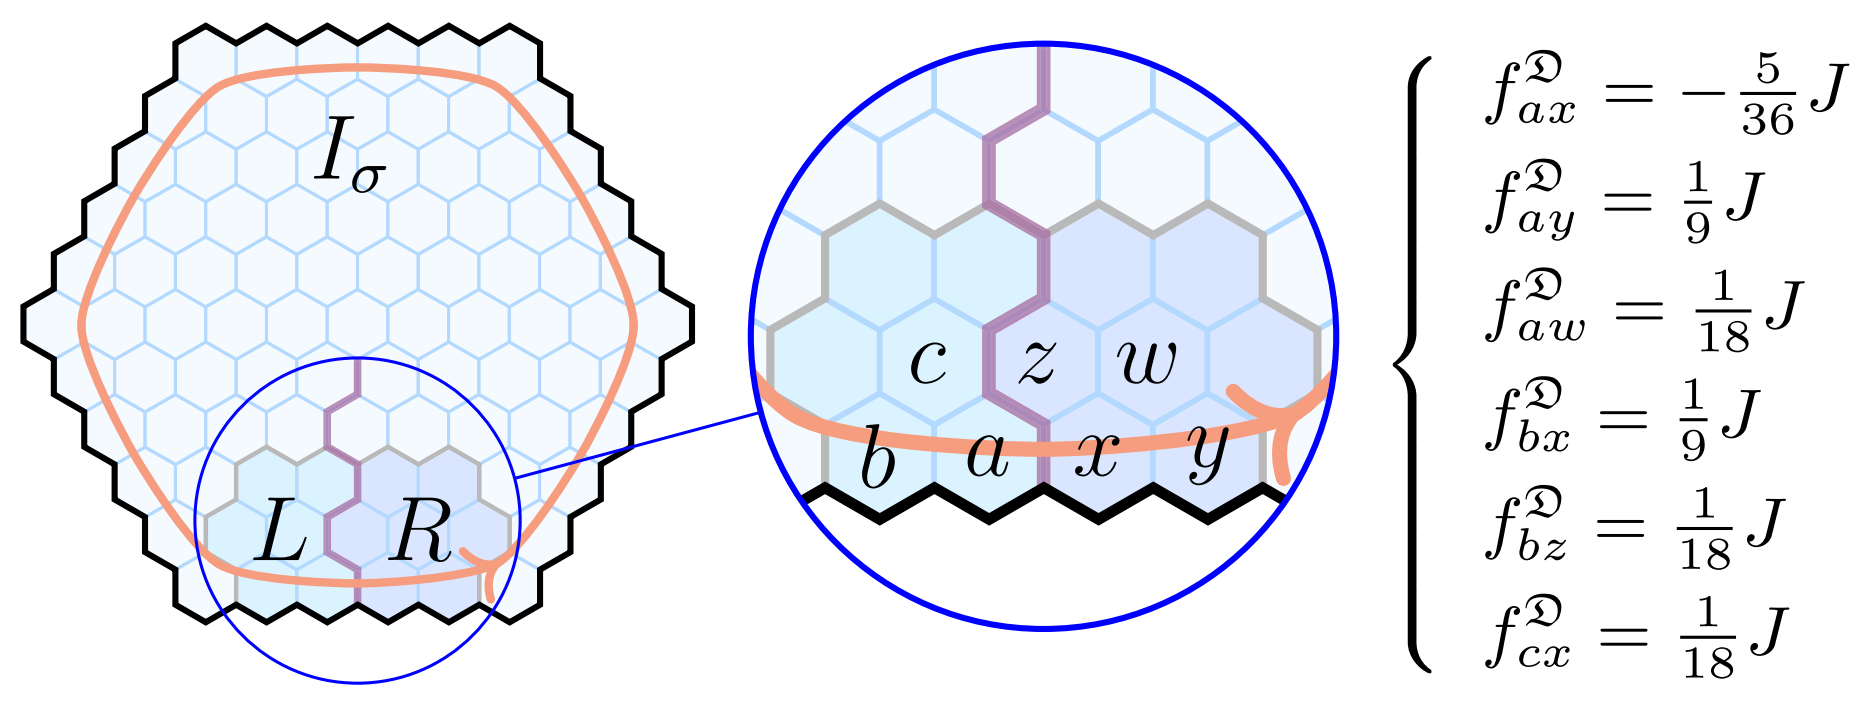
\includegraphics[height=0.2\linewidth]{edge-current.png}
\end{figure}
\begin{itemize}
    \item $f_{u\to v}^\mathfrak{D}=0,\quad \forall v,u \in \mathfrak{D}_{\mrm{int}}$. That is, there is only \textbf{edge current}.
    \item Every modular commutator can be reduced to $J \equiv J\lr{\wordfig{0.7}{elementary-face}}$.
    \item The edge current can be calculated: $I_\sigma\equiv \sum_{u\in L}\sum_{v\in R}f_{u\to v}^\mathfrak{D} = \frac{1}{4}J$
    \item The edge modular current should have the same form as the energy current, $I_\sigma = I(T=1) = \left.\frac{\pi}{12}c_-T^2\right|_{T=1}$
    \item $J = \frac{\pi}{3}c_-$ , a formula relates CCC to the ground state entanglement.
\end{itemize}
\end{frame}
%%%%%%%%%%%%%%%%%%%%%%%%%%%%%%%%%%%%%%%%%%%%%%%%
\begin{frame}

\textbf{Conclusions:}
\begin{itemize}
    \item The \textbf{modular commutator} can be treated as a link that bridges the \textbf{many-body entanglement} with the \textbf{chiral central charge (CCC)}.
 
    \item For gapped systems, the area law is suggested to hold, which gives rise to the \textbf{quantum Markov chain} feature of the system.
 
    \item Entanglement Hamiltonians can be decomposed into small pieces via the quantum Markov chain trick, which \textbf{makes the modular commutator topological}.
 
    \item It is conjectured that two gapped Hamiltonians having the same bulk reduced density matrix generate the same edge current $I = \frac{\pi}{12}c_- T^2$.
 
    \item A succinct formula relating the CCC and elementary modular commutator is derived: $J = \frac{\pi}{3}c_-$.
\end{itemize}
 
\textbf{Problems:}
\begin{itemize}
    \item The area law axioms are not guaranteed to hold.
    
    \item Violation of area law
\end{itemize}


    
\end{frame}
%%%%%%%%%%%%%%%%%%%%%%%%%%%%%%%%%%%%%%%%%%%%%%%%
\end{document}

\item The main result relies on $J\lr{\wordfigdir{0.7}{\tikz[scale=0.25,baseline=5ex]{	
		\coloredboxhx{white,opacity=0.5}{6}{2}{7}{2};
			\coloredboxhx{white,opacity=0.5}{7}{3}{7}{3};
			\node at (5,1.73) {$w$};
			\node at (5.5,2.55) {$v$};
			\node at (6,1.73) {$u$};
	} }} = J$, but the elementary face \wordfigdir{0.5}{\tikz[scale=0.25,baseline=5ex]{	
		\coloredboxhx{white,opacity=0.5}{6}{2}{7}{2};
			\coloredboxhx{white,opacity=0.5}{7}{3}{7}{3};
			\node at (5,1.73) {$w$};
			\node at (5.5,2.55) {$v$};
			\node at (6,1.73) {$u$};
	} } might be too small for the axioms to hold.